\subsection{Order-by-order Solution to RGPEP Equation}
\subsubsection{$\mathcal{O}(g)$ Solution}
\label{sec:first-order}
At first order in $g$, the RGPEP equation is 

\begin{equation}
    \label{eq:first-order}
    \frac{dH^{(1)}(t)}{dt} = \left[\left[H_0, H^{(1)}(t) \right], H_0 \right].
\end{equation}

We can see that the inner commutator in equation \ref{eq:first-order} is the same form as the generator, but at first order. 
Thus, we define $\mathcal{G}^{(1)}(t) = \left[H_0,  H^{(1)}(t)\right]$.
The first step in solving equation \ref{eq:first-order}, is by working out this commutator. 
This will also elucidate some structure of this method that will greatly simplify calculations.

The free Hamiltonian term, written in terms of ladder operators given in equations \ref{eq:phi}, \ref{eq:psi} is 

\begin{equation}
    \label{eq:H-free-ladder}
    H_0 = \int_q \frac{m^2}{q^+}\left(b_q^\dagger b_q + d_q^\dagger d_q \right) + \int_q \frac{\mu^2}{q^+}a_q^\dagger a_q,
\end{equation}

where $$\int_q \equiv \int \frac{dq^+}{4\pi}.$$

While too long to write out $H_Y$ in this form, looking at one term in the expansion of $\bar \psi \psi \phi$ in equation \ref{eq:H-3}, and working out its commutator with equation \ref{eq:H-free-ladder} will give the general form of the generator.

One term in \ref{eq:H-3} is $$\int_{q_1 q_2 q_3}C_{q_1, q_2, q_3}(t)\theta(-q_1^+)\theta(q_2^+)\theta(q_3^+) \bar u(-q_1) u(q_2) b_{-q_1}^\dagger b_{q_2} a_{q_3}.$$
The commutator that must be worked out to obtain the corresponding term of $\mathcal{G}^{(1)}(t)$ is

$$
    \left[\int_q \frac{m^2}{q^+}\left(b_q^\dagger b_q + d_q^\dagger d_q \right) + \int_q \frac{\mu^2}{q^+}a_q^\dagger a_q,  \int_{q_1 q_2 q_3}C_{q_1, q_2, q_3}(t)\theta(-q_1^+)\theta(q_2^+)\theta(q_3^+) \bar u(-q_1) u(q_2) b_{-q_1}^\dagger b_{q_2} a_{q_3}\right].
$$

This commutator equals $$\int_{q_1 q_2 q_3}-\left(q_1^- + q_2^- + q_3^- \right)C_{q_1, q_2, q_3}(t)\theta(-q_1^+)\theta(q_2^+)\theta(q_3^+) \bar u(-q_1) u(q_2) b_{-q_1}^\dagger b_{q_2} a_{q_3}.$$
This is simply the original term from $H^{(1)}(t)$ in the commutator, modified by $-\left(q_1^- + q_2^- + q_3^- \right)$, the negative sum of the total momentum flowing into the vertex. 
It turns out that working out the commutator between $H_0$ and every term in $H^{(1)}(t)$ yields this same form.
Thus, the generator, at first order, is simply a modification of the first order Hamiltonian modified by the negative sum of momentum flowing into each vertex:

\begin{equation}
    \mathcal{G}^{(1)}(t) = -\mathcal{Q}^- H^{(1)}(t).
\end{equation}

Now that $\mathcal{G}^{(1)}(t)$ has been worked out, the full right-hand side of equation \ref{eq:first-order} can be determined:

\begin{align*}
    \left[\mathcal{G}^{(1)}(t), H_0 \right] &= \left[-\mathcal{Q}^- H^{(1)}(t), H_0 \right]\\
    &= -\mathcal{Q}^-\left[H^{(1)}(t), H_0 \right]\\
    &= -\mathcal{Q}^- \left(-\mathcal{G}^{(1)}(t) \right)\\
    &= -\left(\mathcal{Q}^-\right)^2H^{(1)}(t).
\end{align*}

Thus, equation \ref{eq:first-order}, in terms of the parameterized coefficient, which then defines $H^{(1)}(t)$ is:

\begin{equation*}
    \frac{dC_{q_1, q_2, q_3}(t)}{dt} = -(q_1^- + q_2^- + q_3^-)^2C_{q_1, q_2, q_3}(t),
\end{equation*}

whose solution, in terms of the Hamiltonian gives:

\begin{equation}
    H^{(1)}(t) = 4\pi g\int_{q_1 q_2 q_3}\delta(q_1^+ + q_2^+ +q_3^+)e^{-t\left(q_1^- + q_2^- + q_3^-\right)^2}:\bar \psi(-q_1) \psi(q_2) \phi(q_3):.
\end{equation}

The exponential term is referred to as a \textit{form factor}, which regulates the 3-point interaction vertices by exponentially damping terms whose energy going into a vertex is large.

% The first order part of $H$ is given in equation \ref{eq:yukawa-hamiltonian}.
% To determine how $H^{(1)}$ evolves in $t$, we must add explicit \textit{t}-dependence to the coefficients of $H^{(1)}$.
% This is done by substituting the coefficients in front of each product of creation and annihilation operators with arbitrary coefficients that depend not only on momenta, but also $t$. 
% For example, the coefficient in front of $b_i^\dagger b_j a_k$ changes from $$4\pi \delta\left(p_i^+ - p_j^+ - p_k^+ \right)\bar u(p_i) u(p_j) \rightarrow c_{ijk}(t)$$  
% The rest of the coefficients can similarly be exchanged for a paramterized version, where it is important to modify the coefficient in a way that it is clear which term it modifies:

% \begin{align}\nonumber
%     4\pi \delta\left(p_i^+ + p_k^+ - p_j^+ \right)\bar{u}(p_i) u(p_j) &\rightarrow c^*_{ikj}(t)\\ \nonumber
%     4\pi \delta\left(p_i^+ - p_j^+ - p_k^+ \right)\bar{v}(p_j) v(p_i) &\rightarrow \bar{c}_{ijk}(t) \\ \nonumber
%     4\pi \delta\left(p_i^+ + p_k^+ - p_j^+ \right)\bar{v}(p_j) v(p_i) &\rightarrow \bar c^*_{ikj}(t)\\ \nonumber
%     4\pi \delta\left(p_i^+ + p_j^+ - p_k^+ \right)\bar{u}(p_i) v(p_j) &\rightarrow \tilde c_{ijk}(t)\\ \nonumber
%     4\pi \delta\left( p_k^+ - p_i^+ - p_j^+ \right)\bar{v}(p_j) u(p_i) &\rightarrow \tilde c^*_{kij}(t)\\ \nonumber
% \end{align}

% The Hamiltonian now assumes a simpler form:

% \begin{align}
%     \label{eq:H-first-order-c-coeffs}
%     H^{(1)}(t) = g\int_i \int_j \int_k &\left(c_{ijk}(t)b_i^\dagger b_j a_k + c_{ikj}^*(t) b_i^\dagger b_j a_k^\dagger + \bar c_{ijk}(t) d_i^\dagger d_j a_k \right. \\ \nonumber
%     & \left. \bar c^*_{ikj}(t) d^\dagger_i d_j a_k^\dagger + \tilde c_{ijk}(t)b_i^\dagger d_j^\dagger a_k + \tilde c^*_{kij}(t) b_i d_j a_k^\dagger \right).
% \end{align}

% where
% \begin{equation}
%     \int_i \rightarrow \int_0^\infty \frac{dp_i^\dagger}{4\pi p_i^+}
% \end{equation}

% We similarly modify the free part of the Hamiltonian as

% \begin{equation}
%     H_0 = \int_n B_n b_n^\dagger b_n + \int_n D_n d_n^\dagger d_n + \int_n A_n a_n^\dagger a_n.
% \end{equation}

% The inner commutator in equation \ref{eq:first-order} modifies each term in the Hamiltonian by the coefficients in the free part $H_0$.
% For example, the first term in equation \ref{eq:H-first-order-c-coeffs} corresponds to fermion $+$ boson in, fermion out. 
% The term thus gets modified by $\left(B_i - D_j - A_k\right)$.
% Continuing this with every term arrives at:

% \begin{align}
%     \label{eq:first-order-inner-commutator}
%     \left[H_0, H^{(1)}(t) \right] &= g\int_i \int_j \int_k \left(\left(B_i - B_j - A_k \right)c_{ijk}(t)b_i^\dagger b_j a_k + \left(B_i + A_k - B_j\right)c_{ikj}^*(t) b_i^\dagger b_j a_k^\dagger + \left(D_i - D_j - A_k \right)\bar c_{ijk}(t) d_i^\dagger d_j a_k \right. \\ \nonumber
%     & \left. \left(D_i + A_k - D_j\right)\bar c^*_{ikj}(t) d^\dagger_i d_j a_k^\dagger + \left(B_i + D_j - A_k\right)\tilde c_{ijk}(t)b_i^\dagger d_j^\dagger a_k + \left(A_k - B_i - D_j \right)\tilde c^*_{kij}(t) b_i d_j a_k^\dagger \right).
% \end{align}

% To get the full right hand side of equation \ref{eq:first-order}, we do another commutator of equation \ref{eq:first-order-inner-commutator} with $H_0$, which gives another factor of the modificiations of the form $B_i + D_j - A_k$, with a negative sign ($H_0$ is on the right of the commutator now). 

% \begin{align}
%     \label{eq:RHS-first-order}
%     \left[\left[H_0, H^{(1)}(t) \right], H_0\right] = g\int_i \int_j \int_k &\left(-\left(B_i - B_j - A_k \right)^2c_{ijk}(t)b_i^\dagger b_j a_k - \left(B_i + A_k - B_j\right)^2c_{ikj}^*(t) b_i^\dagger b_j a_k^\dagger \right. \\ \nonumber
%     &\left. - \left(D_i - D_j - A_k \right)^2\bar c_{ijk}(t) d_i^\dagger d_j a_k -\left(D_i + A_k - D_j\right)^2\bar c^*_{ikj}(t) d^\dagger_i d_j a_k^\dagger\right. \\ \nonumber
%     & \left.  - \left(B_i + D_j - A_k\right)^2\tilde c_{ijk}(t)b_i^\dagger d_j^\dagger a_k - \left(A_k - B_i - D_j \right)^2\tilde c^*_{kij}(t) b_i d_j a_k^\dagger \right).
% \end{align}

% If we differentiate equation \ref{eq:H-first-order-c-coeffs}, the coefficients in $t$ now become derivatives in $t$.
% Term by term, we can equate the derivatives on the left hand side of \ref{eq:first-order} with the corresponding term from equation \ref{eq:RHS-first-order}.
% For example, 

% \begin{equation}
%     \frac{d}{dt}c_{ijk}(t) = -\left(B_i - B_j - A_k \right)^2 c_{ijk}(t)
% \end{equation}

% which has solution 

% \begin{equation}
%     c_{ijk}(t) = c_{ijk}(0)e^{-\left(B_i - B_j - A_k \right)^2t}
% \end{equation}
% where $c_{ijk}(0)$ comes from the initial Hamiltonian we wrote down: $c_{ijk}(0) = 4\pi \delta\left(p_i^+ - p_j^+ - p_k^+ \right)\bar u(p_i) u(p_j)$.
% Thus, the full first order solution is given as:
 
% \begin{align}
%     &H^{(1)}(t) = \int_0^\infty\int_0^\infty\int_0^\infty \frac{dp_i^+dp_j^+dp_k^+}{\left(4\pi \right)^3 p_i^+ p_j^+ p_k^+}\left(4\pi \delta\left(p_i^+ - p_j^+ - p_k^+ \right) \bar u(p_i) u(p_j) e^{-\left(\frac{m_F^2}{p_i^+} - \frac{m_F^2}{p_j^+} - \frac{m_B^2}{p_k^+} \right)^2t} b_i^\dagger b_j a_k \right.\\ \nonumber
%     &\left. +4\pi \delta\left(p_i^+ + p_k^+- p_j^+  \right) \bar u(p_i) u(p_j) e^{-\left(\frac{m_F^2}{p_i^+} + \frac{m_B^2}{p_k^+} - \frac{m_F^2}{p_j^+}  \right)^2t} b_i^\dagger b_j a_k^\dagger + 4\pi \delta\left(p_i^+ - p_j^+ - p_k^+ \right) \bar v(p_j) v(p_i) e^{-\left(\frac{m_{\bar F}^2}{p_i^+} - \frac{m_{\bar F}^2}{p_j^+} - \frac{m_B^2}{p_k^+} \right)^2t} d_i^\dagger d_j a_k \right. \\ \nonumber
%     &\left.  +4\pi \delta\left(p_i^+ + p_k^+ - p_j^+ \right) \bar v(p_j) v(p_i) e^{-\left(\frac{m_{\bar F}^2}{p_i^+} + \frac{m_B^2}{p_k^+} - \frac{m_{\bar F}^2}{p_j^+}  \right)^2t} d_i^\dagger d_j a_k^\dagger + 4\pi \delta\left(p_i^+ + p_j^+ - p_k^+ \right) \bar u(p_i) v(p_j) e^{-\left(\frac{m_F^2}{p_i^+} + \frac{m_{\bar F}^2}{p_j^+} - \frac{m_B^2}{p_k^+} \right)^2t} b_i^\dagger d_j^\dagger a_k \right. \\ \nonumber
%     & \left.  +4\pi \delta\left(p_i^+ + p_j^+ - p_k^+ \right) \bar v(p_j) u(p_i) e^{-\left(\frac{m_B^2}{p_k^+} - \frac{m_F^2}{p_i^+} - \frac{m_{\bar F}^2}{p_j^+}  \right)^2t}b_i d_j a_k^\dagger\right)\\ \nonumber
% \end{align}

% It is important to note that the exponentials in $t$ are referred to as \textit{form factors}.

% \subsubsection{$\mathcal{O}(g^2)$ Solution}
% \label{sec:second-order}
% At second order in $g$, the RGPEP equation is more involved:

% \begin{equation}
%     \label{eq:rgpep-second-order}
% g^2\dot{H}^{(2)}(t) = \left[\left[H_0, g^2H^{(2)}(t)\right], H_0\right] + \left[\left[H_0, gH^{(1)}(t)\right],gH^{(1)}(t)\right]
% \end{equation}

% At first glance at equation \ref{eq:yukawa-hamiltonian}, it appears as if only the instantaneous terms make up $H^{(2)}(t)$. 
% However, it is important to add to $H^{(2)}(t)$ higher order terms arising from combining two $\mathcal{O}(g)$ interactions. 
% Computing the second commutator in equation \ref{eq:rgpep-second-order} reveals the $\mathcal{O}(g^2)$ interaction terms. 
% This commutator is written as $$\left[\mathcal{G}^{(1)}(t), H^{(1)}(t) \right].$$
% Using Wick's theorem, we can simplify this commutator \footnote{For example, to compute $\left[b_n^\dagger b_n, b_x^\dagger b_y a_z \right] = b_n^\dagger b_nb_x^\dagger b_y a_z - b_x^\dagger b_y a_zb_n^\dagger b_n$, we first normal order both terms and induce Dirac deltas: $b_n^\dagger b_nb_x^\dagger b_y a_z - b_x^\dagger b_y a_zb_n^\dagger b_n = b_n^\dagger \left(\delta_{nx} - b_x^\dagger b_n \right)b_y a_z - b_x^\dagger \left(\delta_{ny} - b_n^\dagger b_y \right)b_n a_z = \delta_{nx}b_n^\dagger b_y a_z - \delta_{ny}b_x^\dagger b_n a_z$. This is the difference between normal ordered contractions in the last line of equation \ref{eq:commutator-to-contractions}}: 

% \begin{align}
%     \label{eq:commutator-to-contractions}
%     \left[\mathcal{G}^{(1)}(t), H^{(1)}(t) \right] &= \mathcal{G}^{(1)}(t)H^{(1)}(t) - H^{(1)}(t)\mathcal{G}^{(1)}(t)\\ \nonumber
%     &= :\mathcal{G}^{(1)}(t)H^{(1)}(t): + :C\left(\mathcal{G}^{(1)}(t)H^{(1)}(t)\right): - :H^{(1)}(t)\mathcal{G}^{(1)}(t): - :C\left(H^{(1)}(t)\mathcal{G}^{(1)}(t) \right):\\ \nonumber
%     &=:C\left(\mathcal{G}^{(1)}(t)H^{(1)}(t)\right): - :C\left(H^{(1)}(t) \mathcal{G}^{(1)}(t)\right):.\\ \nonumber
% \end{align} 

% Here, it is assumed that $:\mathcal{G}^{(1)}(t)H^{(1)}(t): = H^{(1)}(t)\mathcal{G}^{(1)}(t): $ since the number of fermions (antifermions) always come in pairs in any quantum field theory.

% We can continue simplifying equation \ref{eq:commutator-to-contractions}:

% \begin{align}
%     \label{eq:full-simplification-of-GH-comm}
%     \left[\mathcal{G}^{(1)}(t), H^{(1)}(t) \right] &= :C\left(\mathcal{G}^{(1)}(t)H^{(1)}(t)\right): - :C\left(H^{(1)}(t) \mathcal{G}^{(1)}(t)\right):\\ \nonumber
%     &= \sum_{D_1, D_2} \left(:C\left(\mathcal{G}_{D_1}^{(1)}(t)H_{D_2}^{(1)}(t)\right): - :C\left(H^{(1)}_{D_1}(t) \mathcal{G}^{(1)}_{D_2}(t)\right) \right) \\ \nonumber
%     &= \sum_{contractions} \left(\mathcal{P}_A + \mathcal{P}_B -2\mathcal{P}_C  \right)V_1(0) V_2(0)T_{contraction}
% \end{align}

% To understand the final form of equation \ref{eq:full-simplification-of-GH-comm}, we note $D_i \in \{\text{Yukawa interactions} \}$. 
% Thus, we calculate contractions of every pair of interaction terms in $H^{(1)}(t)$ (since interaction terms in $\mathcal{G}^{(1)}(t)$ are the same, up to some coefficient modifications).
% After writing down every possible contraction, we now have $\mathcal{O}(g^2)$ interaction diagrams, labeled by $T_{contraction}$, which describes the ladder operator structure of the term. 
% Instead of meticulously keeping track of indices, the last line in equation \ref{eq:full-simplification-of-GH-comm} allows you to take a given contraction from two interactions, and gives the modification to the coefficient needed to write out the commutator in equation \ref{eq:full-simplification-of-GH-comm}.
% An example is given in figures \ref{fig:D1D2} and \ref{fig:contraction}.

% % \begin{figure}
% %     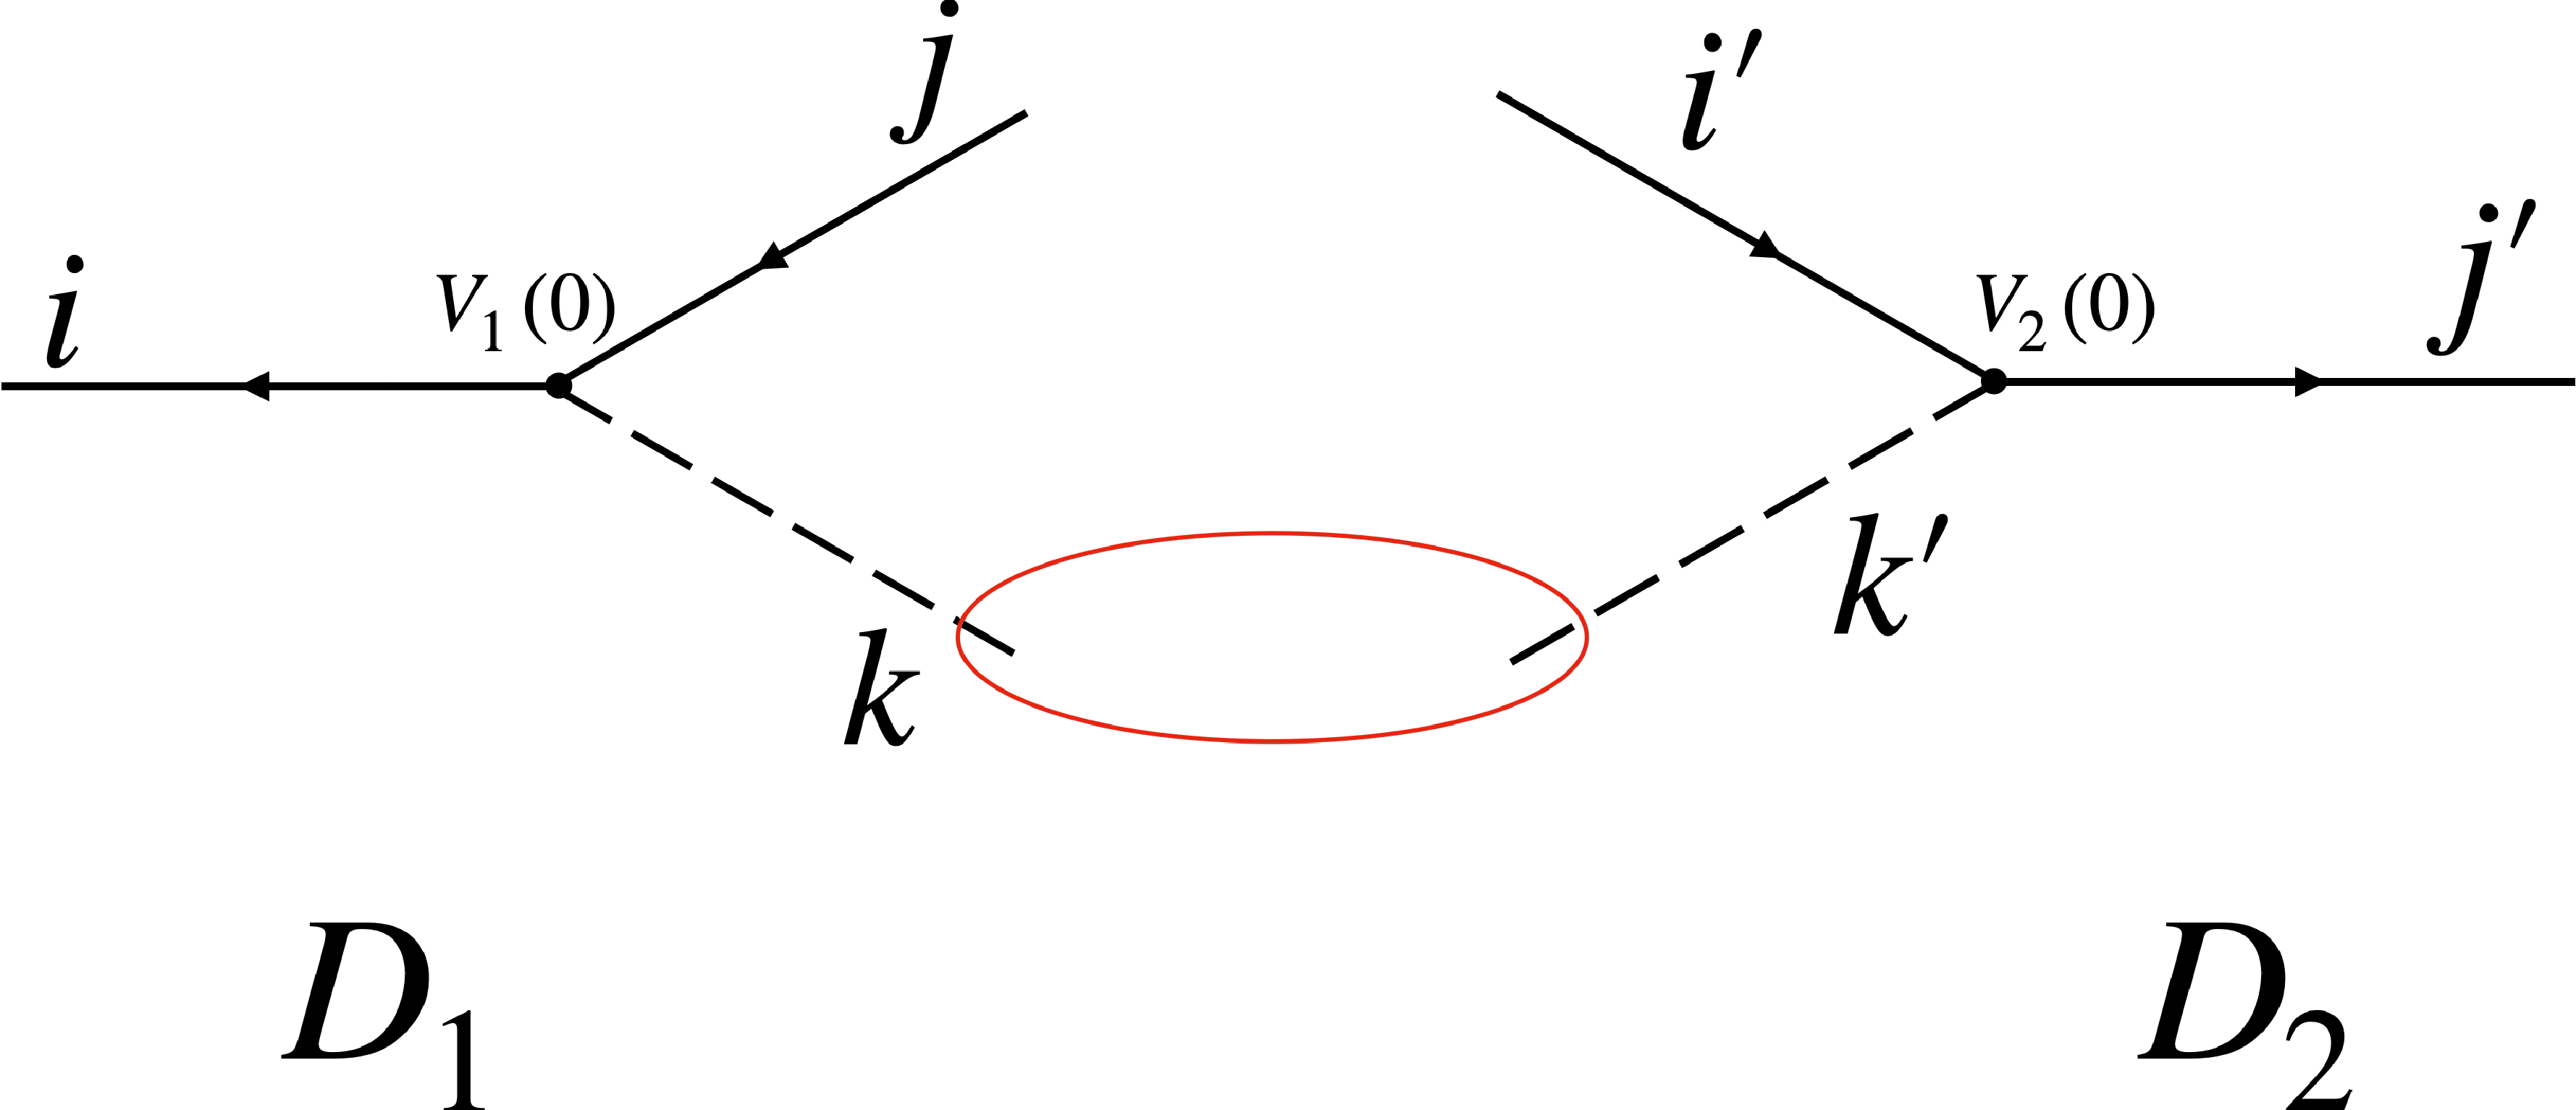
\includegraphics[width = 0.75\textwidth]{figures/D1D2.pdf}
% %     \caption{Two interaction diagrams, $D1$ and $D2$ are chosen. There is only one possible contraction, which is circled in red.}
% %     \label{fig:D1D2}
% % \end{figure}

% % \begin{figure}
% %     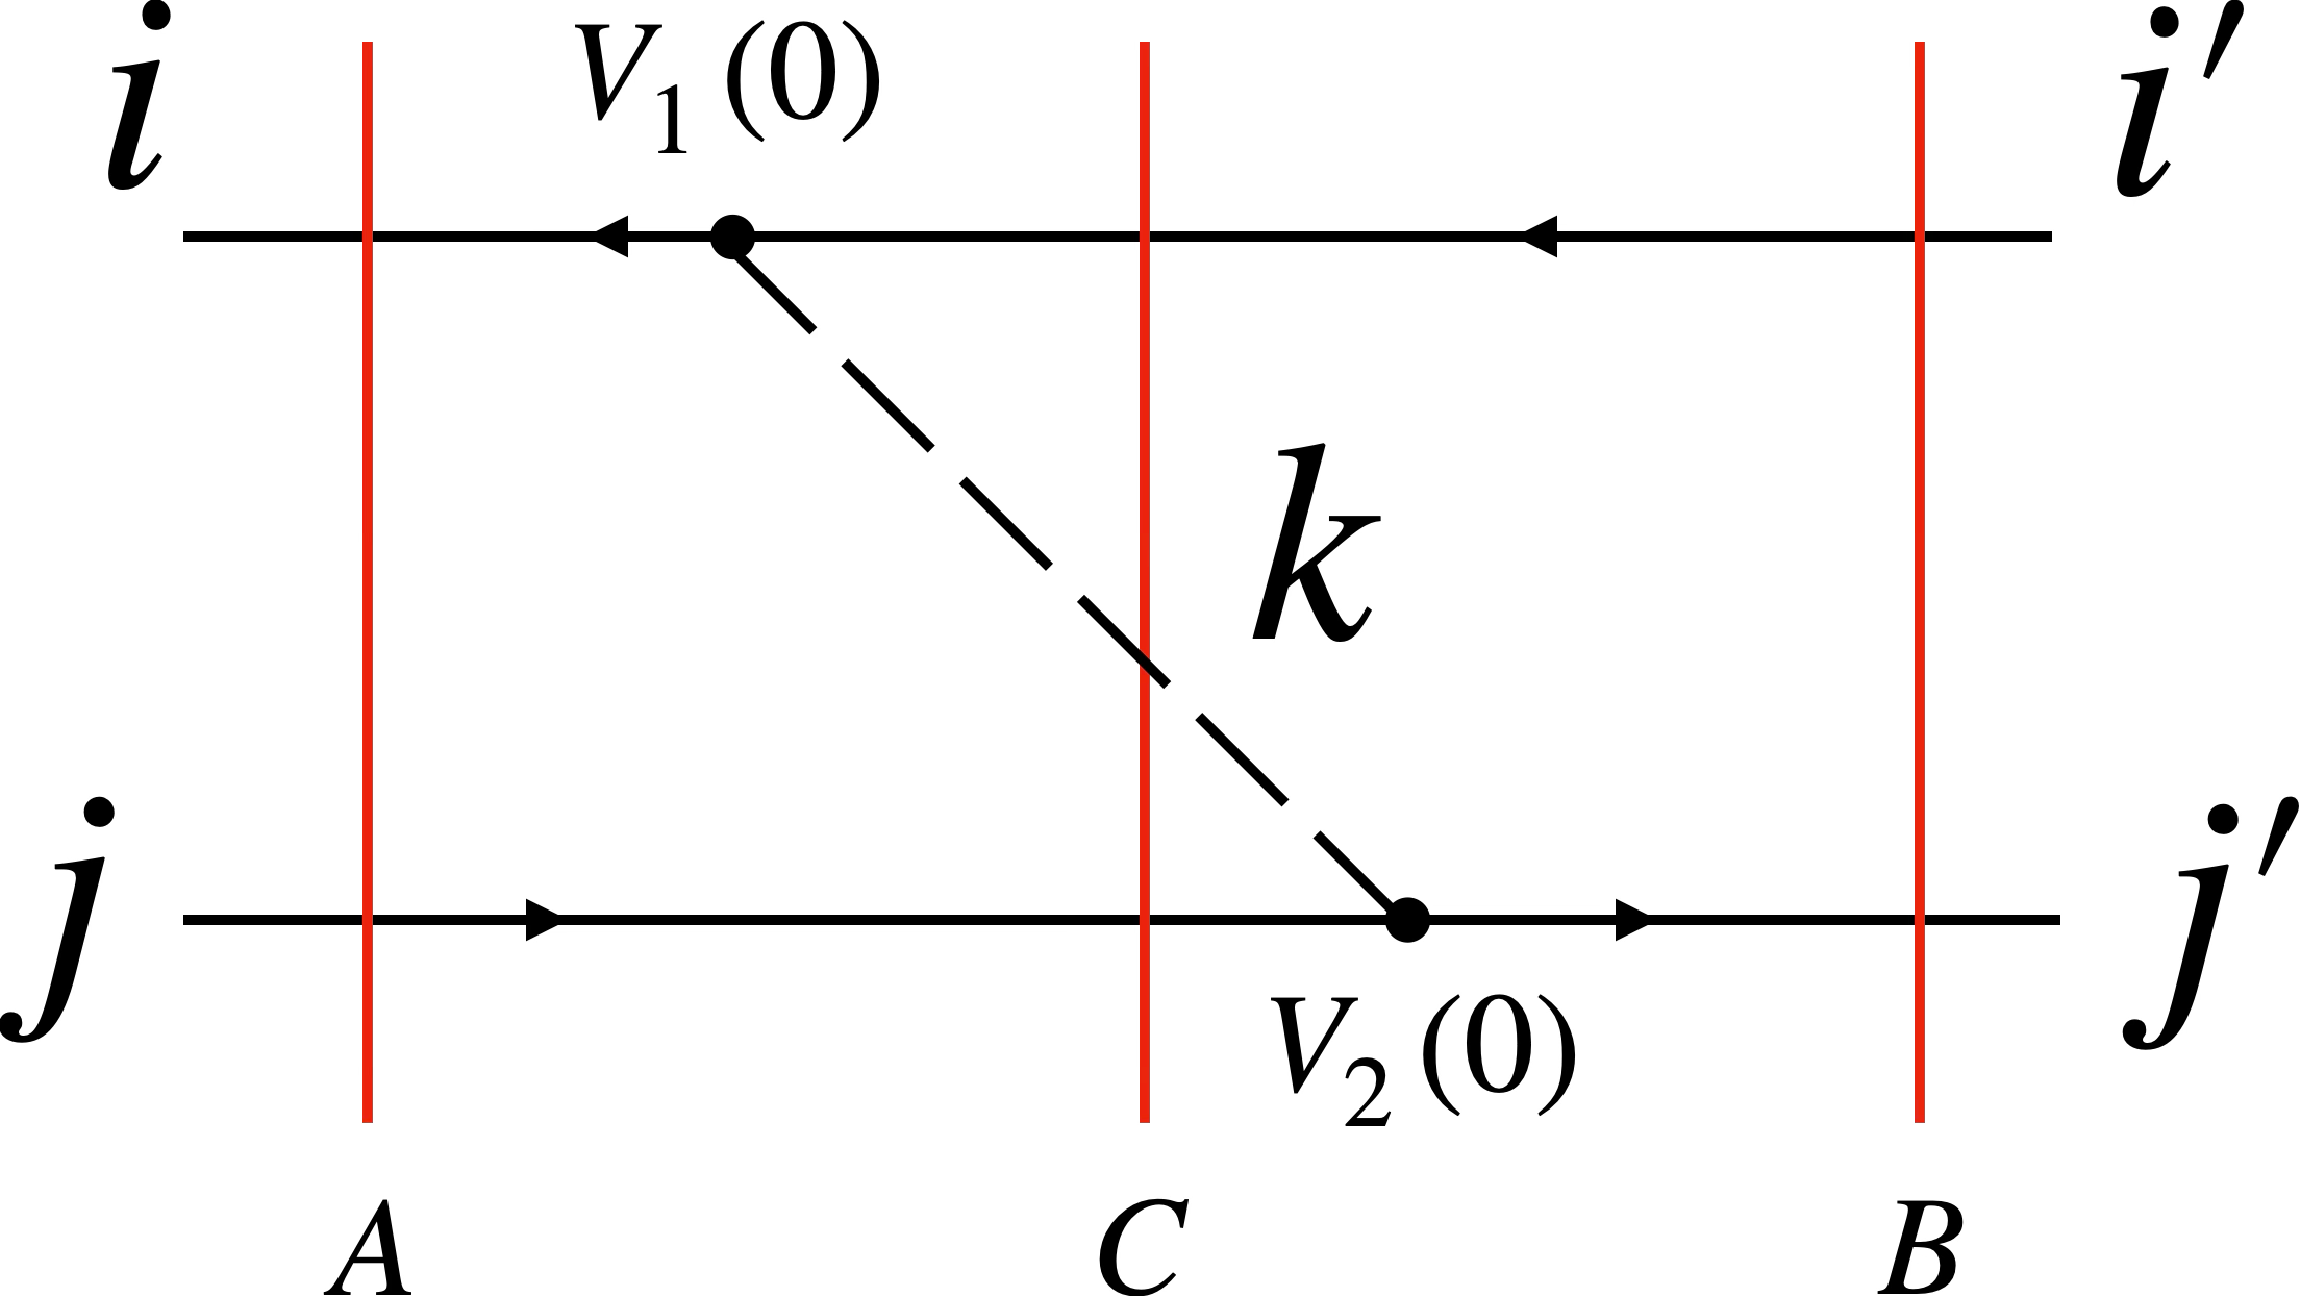
\includegraphics[width = 0.6\textwidth]{figures/contraction.pdf}
% %     \caption{When we contract the bosons in $D1$ and $D2$ in figure \ref{fig:D1D2}, we get an $\mathcal{O}(g^2)$ diagram. Keeping track of the original indices is unnecesssary, if you label them in a consistent way.}
% %     \label{fig:contraction}
% % \end{figure}

% For this example, $\mathcal{P}_A + \mathcal{P}_B - 2\mathcal{P}_2 = c_i - c_{i'} + c_j - c_{j'} - 2c_k$ (i.e. $\mathcal{P}_i$ is the sum of momentum along the red line of $i$), and $V_1(t) = c_{ijk}(t), V_2(t) = \bar c^*_{ijk}(t)$. Thus, $$\left[\mathcal{G}^{(1)}(t), H^{(1)}(t) \right]_{D_1, D_2} = \int_{ijki'j'}\left(c_i - c_{i'} + c_j - c_{j'} - 2c_k \right)c_{ijk}(0)\bar c^*_{ijk}(0) b_i^\dagger b_{i'}d_j^\dagger d_{j'}.$$

% Doing this $\forall D_1, D_2 \in \{interactions\}$, we obtain $\left[\mathcal{G}^{(1)}(t), H^{(1)}(t) \right]$. 
% The important information obtained from computing all of the contractions is that you can now write down a parameterized form for $\mathcal{O}(g^2)$ terms to add to $H^{(2)}(t)$. 
% Again, using the example of figures \ref{fig:D1D2} and \ref{fig:contraction}, we could parameterize this addition to $H^{(2)}(t)$ as $$H^{(2)}_{D_1, D_2}(t) = \int_{ijki'j'}K(t)  b_i^\dagger b_{i'}d_j^\dagger d_{j'},$$ where $K(t)$ is a parameterized coefficient to be determined by solving equation \ref{eq:rgpep-second-order}. \gus{Change $D1, D2$ subscript in above equation to be a figure of the corresponding diagram}.

% Now that we have a parameterized form of $H^{(2)}(t)$, complete with additional terms from the contractions, we can calculate the first commutator in equation \ref{eq:rgpep-second-order}.

% For a given term in $H^{(2)}(t)$, the commutator $\left[\left[H_0, g^2H^{(2)}(t)\right], H_0\right]$ is simple to calculate. 
% In a similar way that $\left[\left[H_0, gH^{(1)}(t)\right], H_0\right]$ was calculated, this second order commutator will modify the given term by $-\left(\mathcal{P}_A - \mathcal{P}_B\right)^2$ (refer to figure \ref{fig:contraction}).

% We can finally write down the general form of the differential equation that comes from equation \ref{eq:rgpep-second-order} for a given second order diagram $D$ with parameterized coefficient in $H^{(2)}(t)$, $K(t)$:

% \begin{equation}
%     \label{eq:second-order-DE}
%     \frac{d}{dt}K_D(t) = -\left(\mathcal{P}_A - \mathcal{P}_B \right)^2 K_D(t) + \left(\mathcal{P}_A + \mathcal{P}_B - 2\mathcal{P}_C \right)V_1(0)e^{-p_{V_1}^2t}V_2(0)e^{-p_{V_2}^2t}
% \end{equation}

% where $p_{V_i}^2$ is sum of $c_j's$ into $V_i$ minus sum of $c_j's$ out of $V_i$. 
% For the example of $D_1$ in figure \ref{fig:D1D2}, $p_{V_1} = \left(c_i - c_j - c_k \right)$.

% The general solution to equation \ref{eq:second-order-DE} is \footnote{A differential equation of the form $\frac{dy}{dt} = -p(t)y(t) + q(t)$ has the general solution $y(t) = e^{-h(t)}\int e^{h(t)}q(t) + Ce^{-h(t)}$, where $h(t) = \int dt p(t)$}:

% \begin{equation}
%     K_D(t) = \frac{\left(\mathcal{P}_A + \mathcal{P}_B - 2\mathcal{P}_C \right)V_1(0)V_2(0)}{p_{V_1}^2 + p_{V_2}^2 - \left(\mathcal{P}_A - \mathcal{P}_B \right)^2} \left(e^{-\left( \mathcal{P}_A - \mathcal{P}_B\right)^2t} - e^{-\left(p_{V_1}^2 + p_{V_2}^2\right)t} \right) + K_D(0)
% \end{equation}

% The last thing to note before writing out the solution to \ref{eq:rgpep-second-order} is that we must take into account the original instantaneous second order diagrams present in \ref{eq:yukawa-hamiltonian}. 
% The first commutator in \ref{eq:rgpep-second-order} will be non-zero for this interaction, and can simply be wrote down as the original term, modified by $-\left(\mathcal{P}_A - \mathcal{P}_B \right)^2$. 
% Each second order term in the Hamiltonian is now written out explicitly in table \ref{tab:H2}:

